% Copyright 2007 by Till Tantau
%
% This file may be distributed and/or modified
%
% 1. under the LaTeX Project Public License and/or
% 2. under the GNU Public License.
%
% See the file doc/licenses/LICENSE for more details.



\documentclass{beamer}

%
% DO NOT USE THIS FILE AS A TEMPLATE FOR YOUR OWN TALKS�!!
%
% Use a file in the directory solutions instead.
% They are much better suited.
%


% Setup appearance:

\usetheme{Darmstadt}
\usefonttheme[onlylarge]{structurebold}
\setbeamerfont*{frametitle}{size=\normalsize,series=\bfseries}
\setbeamerfont*{page number in head}{size=\large}
\setbeamertemplate{navigation symbols}{}
\setbeamertemplate{footline}[frame number]
\setbeamertemplate{caption}[numbered]
% Standard packages

\usepackage[english]{babel}
\usepackage[latin1]{inputenc}
\usepackage{times}
\usepackage[T1]{fontenc}
\usepackage{enumitem}
\setitemize{label=\usebeamerfont*{itemize item}
  \usebeamercolor[fg]{itemize item}
  \usebeamertemplate{itemize item}}
\usepackage{booktabs}
% Setup TikZ
\usepackage{xcolor}
\usepackage{tikz}
\usetikzlibrary{arrows}
\tikzstyle{block}=[draw opacity=0.7,line width=1.4cm]


% Author, Title, etc.

\title[ Distributed $3$D-Print Driver] 
{%
  Distributed \textbf{$3$}D-Print Driver
 %
}

\author[Guide]{
	\textbf{Presenter}: Suman~Bidarahalli \\
	\textbf{Supervisors}: \\
	Prof. Dr. Arjan~Kuijper \\  
	Alan~Brunton	\\ 
	Marco~Dennst{\"a}dt 
}
\institute[TU Darmstadt]
{
  Technische Universit�t Darmstadt, Germany
}

\date[ Master Thesis Presentation 2017]
{Master Thesis Presentation, February 2017}



% The main document

\begin{document}

\begin{frame}
  \titlepage
\end{frame}

\begin{frame}{Outline}
  \tableofcontents
\end{frame}


\section{Introduction}

\subsection{State of the art $3$D Printers}

\begin{frame}{Motivation}

\begin{columns}
    \begin{column}{0.25\textwidth}
    \centering
    \begin{figure}[!ht]
			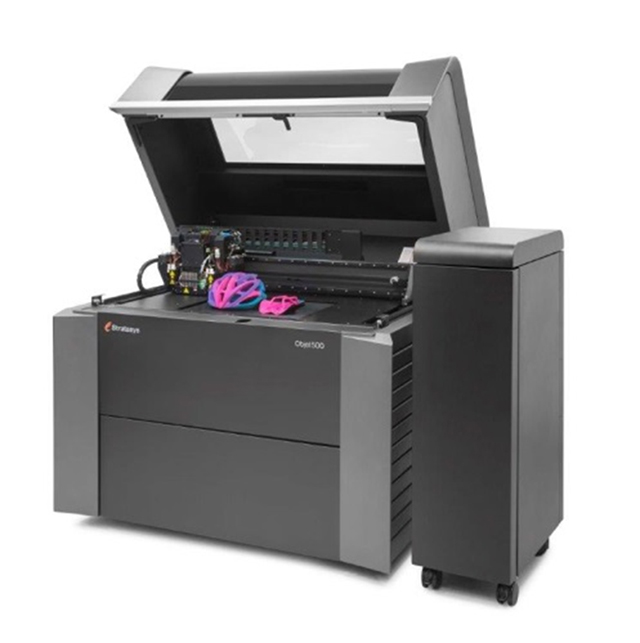
\includegraphics[width=0.90\textwidth]{PrinterI}
			\caption{State of the art $3$D Printers}
			\label{Fig:State of the art $3$D Printers}
		\end{figure}
    \end{column}
    \begin{column}{0.75\textwidth}
    \centering
    \begin{itemize}
			\item Total print volume of Connex3 is $\sim$ 360 billion voxels
			\item Multiple print objects in varying size can be printed at a go
		\end{itemize} 
    \end{column}
  \end{columns}
\end{frame}

\subsection{Problem Statement}

\begin{frame}[t]{Requirement and Derived Goals}
\begin{columns}
    \begin{column}{0.40\textwidth}
    \centering
    \begin{figure}[!ht]
			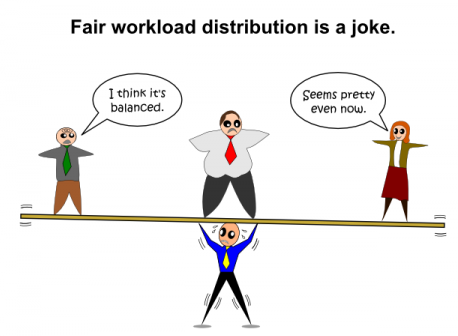
\includegraphics[width=0.90\textwidth]{SillyImage}
			\label{Fig:MythI}
		\end{figure}
    \end{column}
    \begin{column}{0.60\textwidth}
    \centering
    \begin{itemize}
    \item \textbf{Requirement}
		\begin{itemize}
		\item Provide Cuttlefish as a cloud service 
		\end{itemize} 
    \item \textbf{Derived Goals}
		\begin{itemize}
		\item Due application specific limitations, requirement changed to cluster computing \newline
		\item To develop Distributed Cuttlefish with an abstraction layer 
		\end{itemize} 
		\end{itemize} 	
    \end{column}
  \end{columns}
\end{frame}

\section{Solution}
\begin{frame}{Currently used Distributed System}
    \begin{figure}[!ht]
			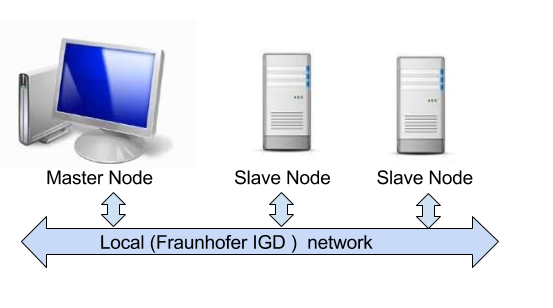
\includegraphics[width=0.80\textwidth]{ArchitectureI.png}
			\caption{Distributed System Architecture}
			\label{Fig:DCArchitecture}
		\end{figure}
\end{frame}

\begin{frame}{Master-Slave Paradigm}
\begin{columns}
  \begin{column}{0.30\textwidth}
  \centering
    \begin{figure}[!ht]
			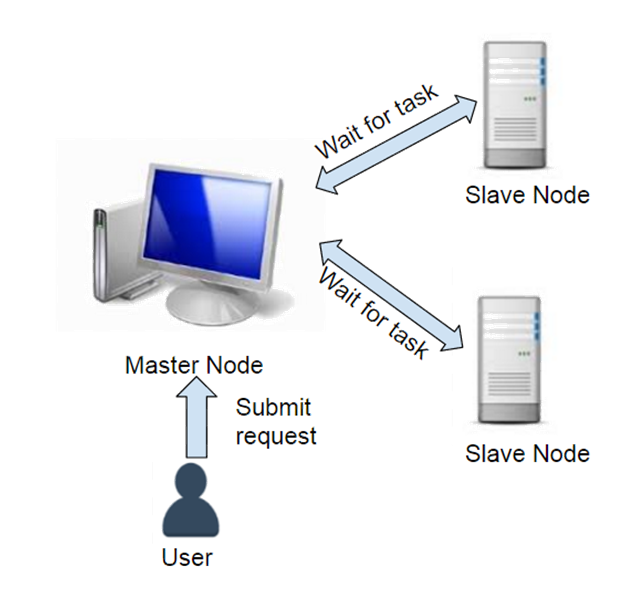
\includegraphics[width=0.90\textwidth]{TaskSubmission.PNG}
			\caption{Step-1:Task Submission}
			\label{Fig:TaskSubmission}
		\end{figure}
	\end{column}
	\begin{column}{0.30\textwidth}
		\begin{figure}[!ht]
			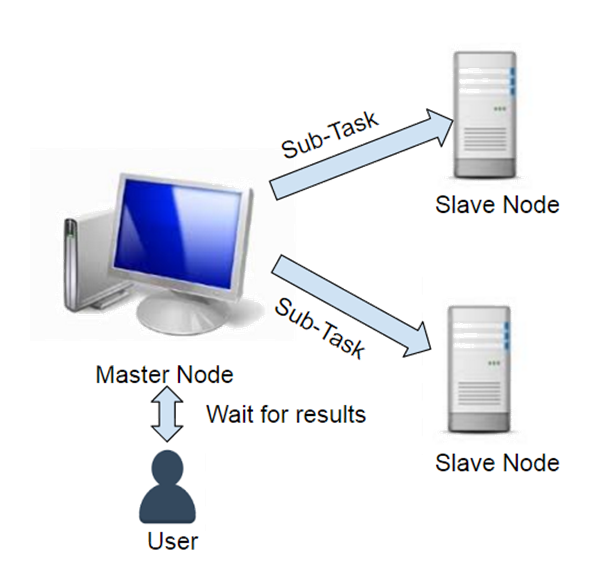
\includegraphics[width=0.90\textwidth]{TaskDistribution.PNG}
			\caption{Step-2: Sub-Task Computation}
			\label{Fig:TaskDistribution}
		\end{figure}
	\end{column}
		\begin{column}{0.30\textwidth}
		\begin{figure}[!ht]
			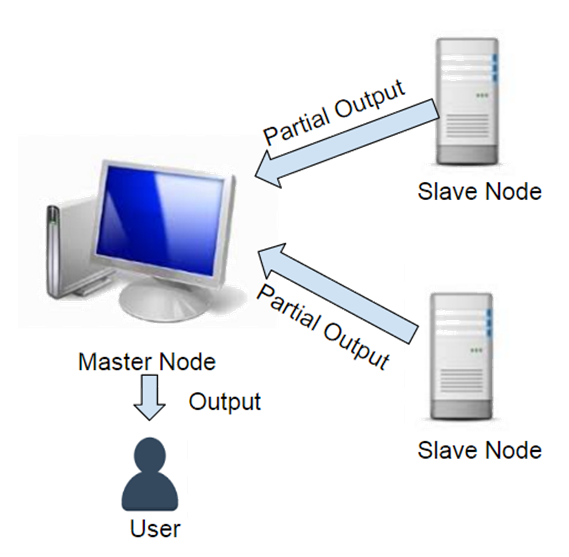
\includegraphics[width=0.90\textwidth]{CollectionAndMerging.PNG}
			\caption{Step-3: Partial Result Collection and Merging}
			\label{Fig:CollectionAndMerging}
		\end{figure}
	\end{column}
\end{columns}
\end{frame}

\subsection{How is the distribution done?}
\begin{frame}{Different possibilities of distribution}
\begin{columns}
   \begin{column}{0.50\textwidth}
    \centering
    \begin{figure}[!ht]
			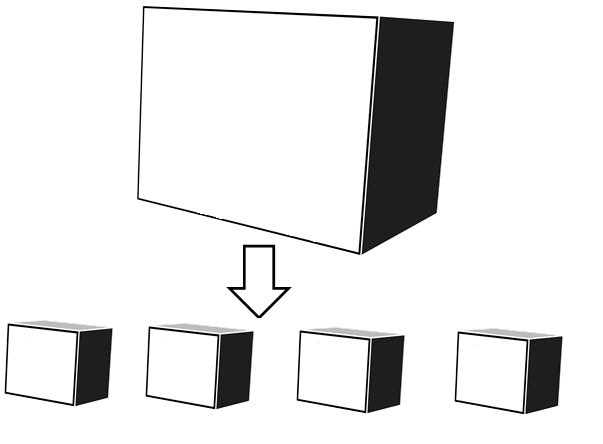
\includegraphics[width=0.90\textwidth]{DistributeI}
			\caption{Distribution of one large print object amongst the workstations }
			\label{Fig:DistributeI}
		\end{figure}
   \end{column}
	\begin{column}{0.50\textwidth}
    \centering
			\begin{figure}[!ht]
			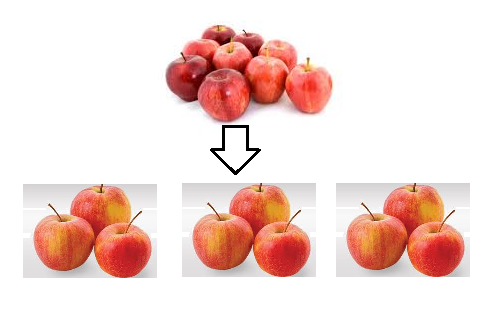
\includegraphics[width=0.90\textwidth]{DistributeII}
			\caption{Distribution of multiple print objects amongst the workstations}
			\label{Fig:DistributeII}
		\end{figure}
    \end{column}
  \end{columns}
  \end{frame}
	
\begin{frame}{Distribution of Sub-Tasks Using Cost Function}
\begin{itemize}
	\item Threshold calculated using the bounding box volume of each object.
	\item Threshold (for cluster size n-1)=\begin{math}(\sum\limits_{i=1}^{k}{V^i})/(n-1)\end{math}
\end{itemize}
\end{frame}	

\subsection{Distributed Cuttlefish Application}
\begin{frame}
\begin{figure}[!ht]
	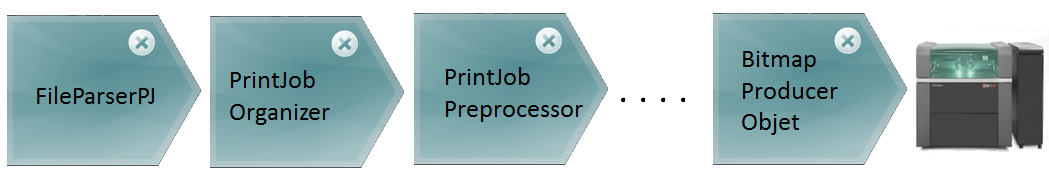
\includegraphics[width=0.9\textwidth]{StreamingArchitectureI.PNG}
	\caption{Cuttlefish Streaming Architecture}
	\label{Fig:CuttlefishPipelineFigure}
\end{figure}
\begin{itemize} 
	\item The computation is performed in a chunk-wise manner 
	\item Enables to start printing the object as soon as the first chunk is processed
\end{itemize} 
\end{frame}

\begin{frame}{Architectural Goals}
	\textbf{Goal}: To \textbf{retain the streaming architecture} by providing distinguished components to handle
	\begin{itemize} 
	\item  Distribution of sub-tasks 
	\item  Distribution of partial results
	\item  Collection of the partial results
	\end{itemize} 
\end{frame}

\begin{frame}{Classification of Prototypes}
	\begin{figure}[!ht]
		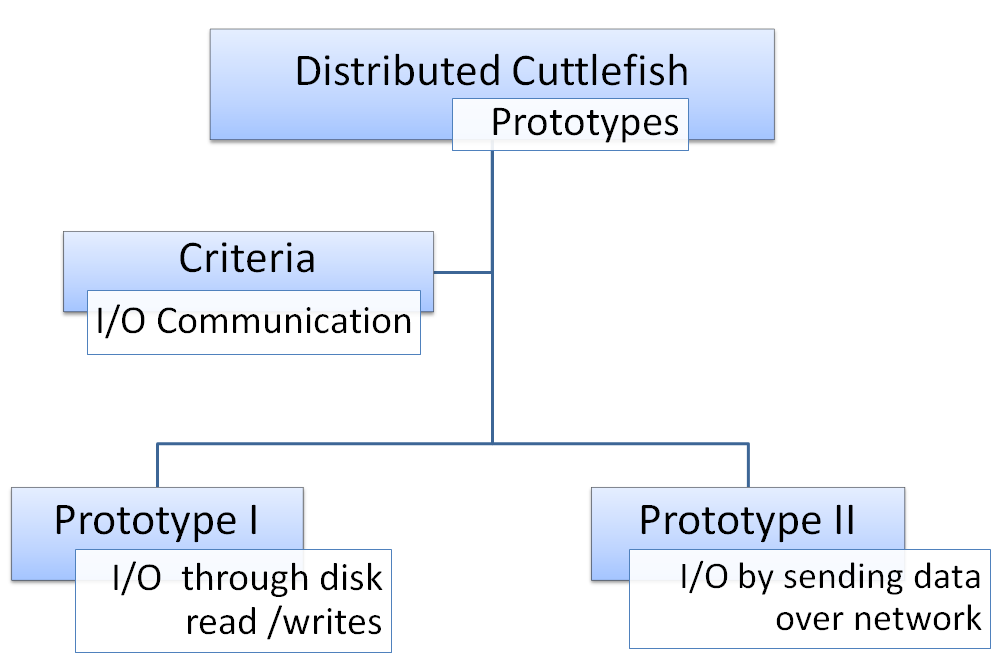
\includegraphics[width=0.9\textwidth]{Prototypes.PNG}
		\caption{Classification of Prototypes}
		\label{Fig:StreamingArchitectureI}
	\end{figure}
\end{frame}

\begin{frame}{Modified Component Architecture- Prototype I}
	\begin{figure}[!ht]
		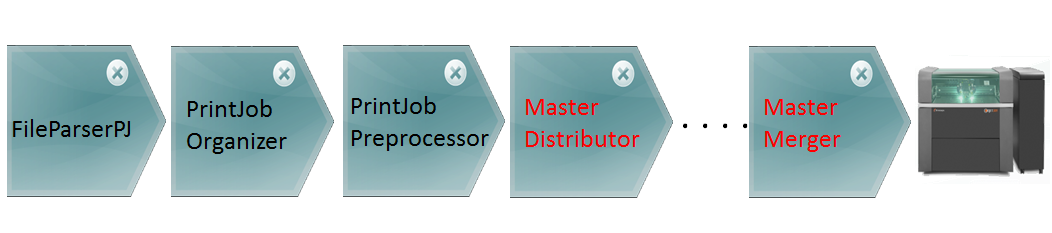
\includegraphics[width=0.9\textwidth]{MSPSPI.png}
		\caption{Master Printing Software}
		\label{Fig:MasterPSPl}
	\end{figure}
	\begin{figure}[!ht]
		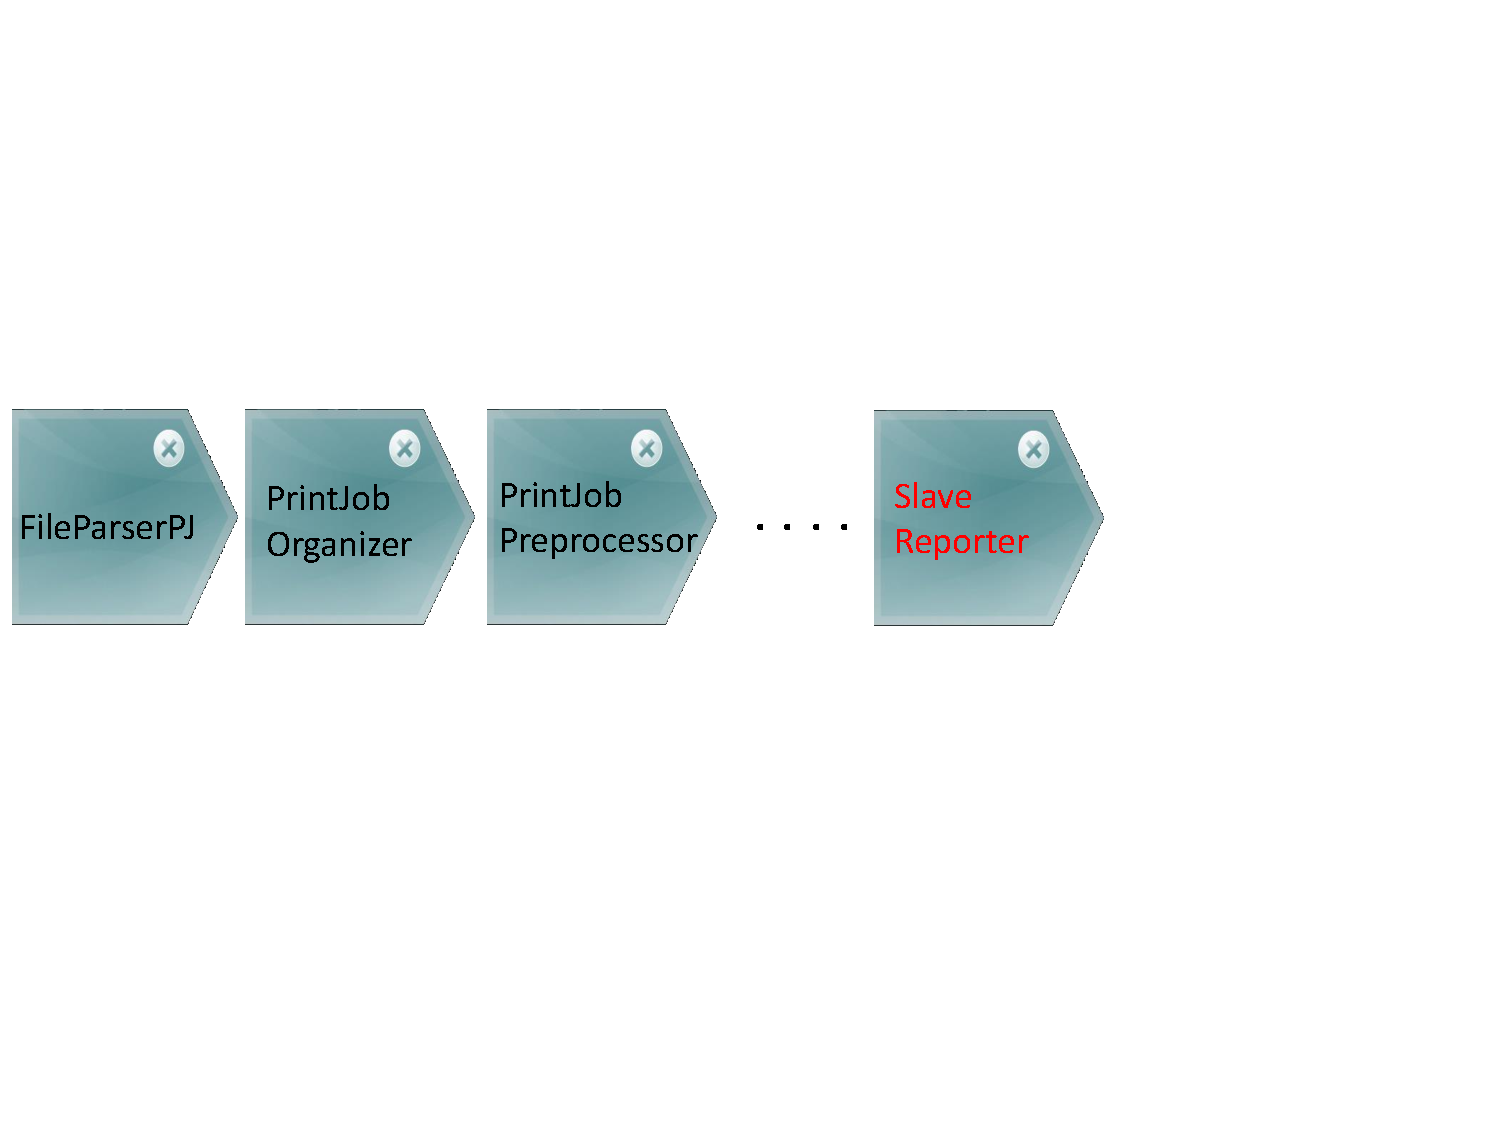
\includegraphics[width=0.8\textwidth]{SlavePSPI.png}
		\caption{Slave Printing Software}
		\label{Fig:SlavePSPI}
	\end{figure}
\end{frame}

\begin{frame}{Modified Component Architecture- Prototype II}
	\begin{figure}[!ht]
		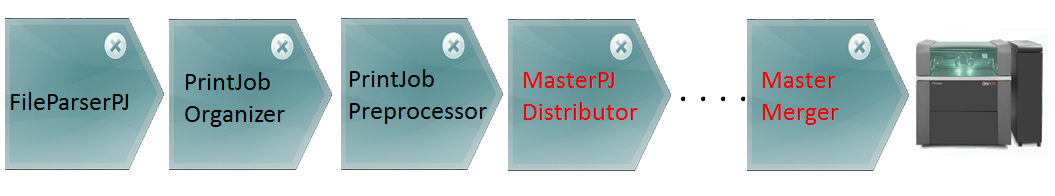
\includegraphics[width=0.9\textwidth]{MSPSPII.png}
		\caption{Master Printing Software}
		\label{Fig:MasterPSPIl}
	\end{figure}
	\begin{figure}[!ht]
		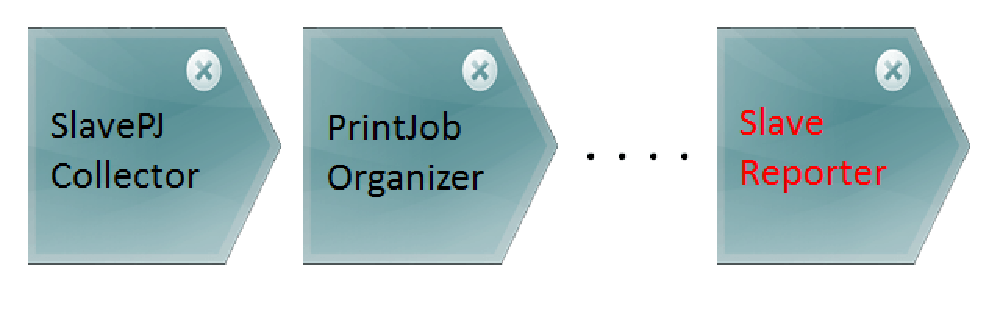
\includegraphics[width=0.7\textwidth]{SlavePSPII.png}
		\caption{Slave Printing Software}
		\label{Fig:SlavePSPII}
	\end{figure}
\end{frame}

\begin{frame}{Abstraction Layer}
	\begin{figure}
		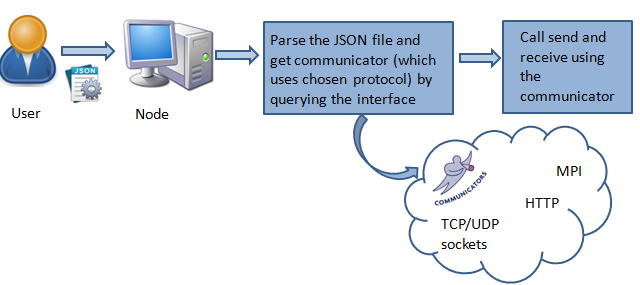
\includegraphics[width=0.9\textwidth]{AbstractionLayer.PNG}
		\caption{Abstraction Layer }
	\end{figure}	
\end{frame}

\begin{frame}{Distributed Computing Tasks}
	\begin{figure}[!ht]
		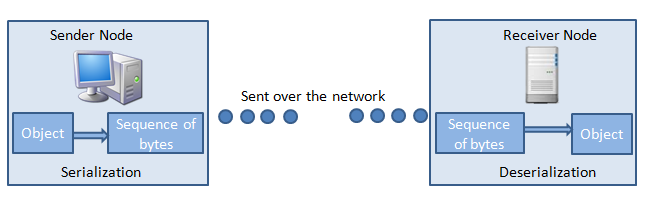
\includegraphics[width=0.7\textwidth]{Ser-Deser.PNG}
		\caption{Serialization And Deserialization }
		\label{Fig:Ser-Deser}
	\end{figure}
	\begin{figure}[!ht]
		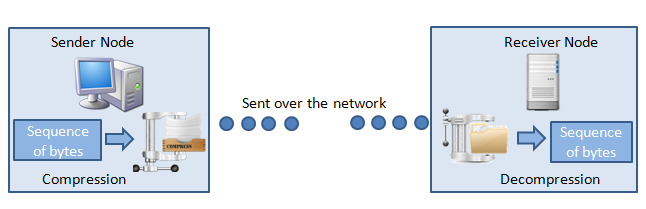
\includegraphics[width=0.7\textwidth]{CompDecomp.PNG}
		\caption{Compression And Decompression }
		\label{Fig:CompDecomp}
	\end{figure}
\end{frame}

\section{Results}
\subsection{Distributed Cuttlefish vs Non-Distributed Cuttlefish}
\begin{frame}
\begin{table}[]
\centering
\scalebox{0.8}{\begin{tabular}{c p{8cm} p{1cm}}
 Model
 & Test Data \\ 
\cmidrule(r){1-1}\cmidrule(lr){2-2}\cmidrule(l){3-3}
\raisebox{-\totalheight}{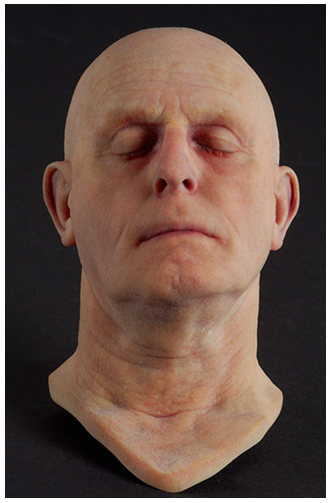
\includegraphics[width=0.2\textwidth]{Head.PNG}}
      & 
\begin{itemize}[topsep=0pt]
\item Head Model Size= 8cm
\item Resolution= \begin{math}300 \times 150 \times 470\end{math}
\item Cluster size= 3 nodes
\end{itemize}
\end{tabular}}
\end{table}

\begin{table}[]
\centering
\caption{Execution Time Comparison}
\label{table:ExecTime}
\scalebox{0.7}{
\begin{tabular}{|l|l|l|l|}
\hline
\multicolumn{1}{|c|}{\textbf{\begin{tabular}[c]{@{}c@{}}Number of \\ Models\end{tabular}}} & \multicolumn{1}{c|}{\textbf{\begin{tabular}[c]{@{}c@{}}Total Execution Time\\  (in Secs)\\ Prototype I\end{tabular}}} & \multicolumn{1}{c|}{\textbf{\begin{tabular}[c]{@{}c@{}}Total Execution Time\\  (in Secs)\\ Prototype II\end{tabular}}} & \multicolumn{1}{c|}{\textbf{\begin{tabular}[c]{@{}c@{}}Total Execution Time \\ (in Secs)\\ Native\\ Cuttlefish\end{tabular}}} \\ \hline
2                                                                                          & 173.35                                                                                                                & 102.55                                                                                                                 & 357.35                                                                                                                        \\ \hline
4                                                                                          & 363.39                                                                                                                & 245.08                                                                                                                 & 920.56                                                                                                                        \\ \hline
6                                                                                          & 585.32                                                                                                                & 440.41                                                                                                                 & 1651.17                                                                                                                       \\ \hline
8                                                                                          & 836.51                                                                                                                & 708.70                                                                                                                 & 4071.56                                                                                                                       \\ \hline
10                                                                                         & 1130.51                                                                                                               & 1014.98                                                                                                                & 4790.19                                                                                                                       \\ \hline
\end{tabular}}
\end{table}
\end{frame}

\begin{frame}
\begin{figure}[!ht]
		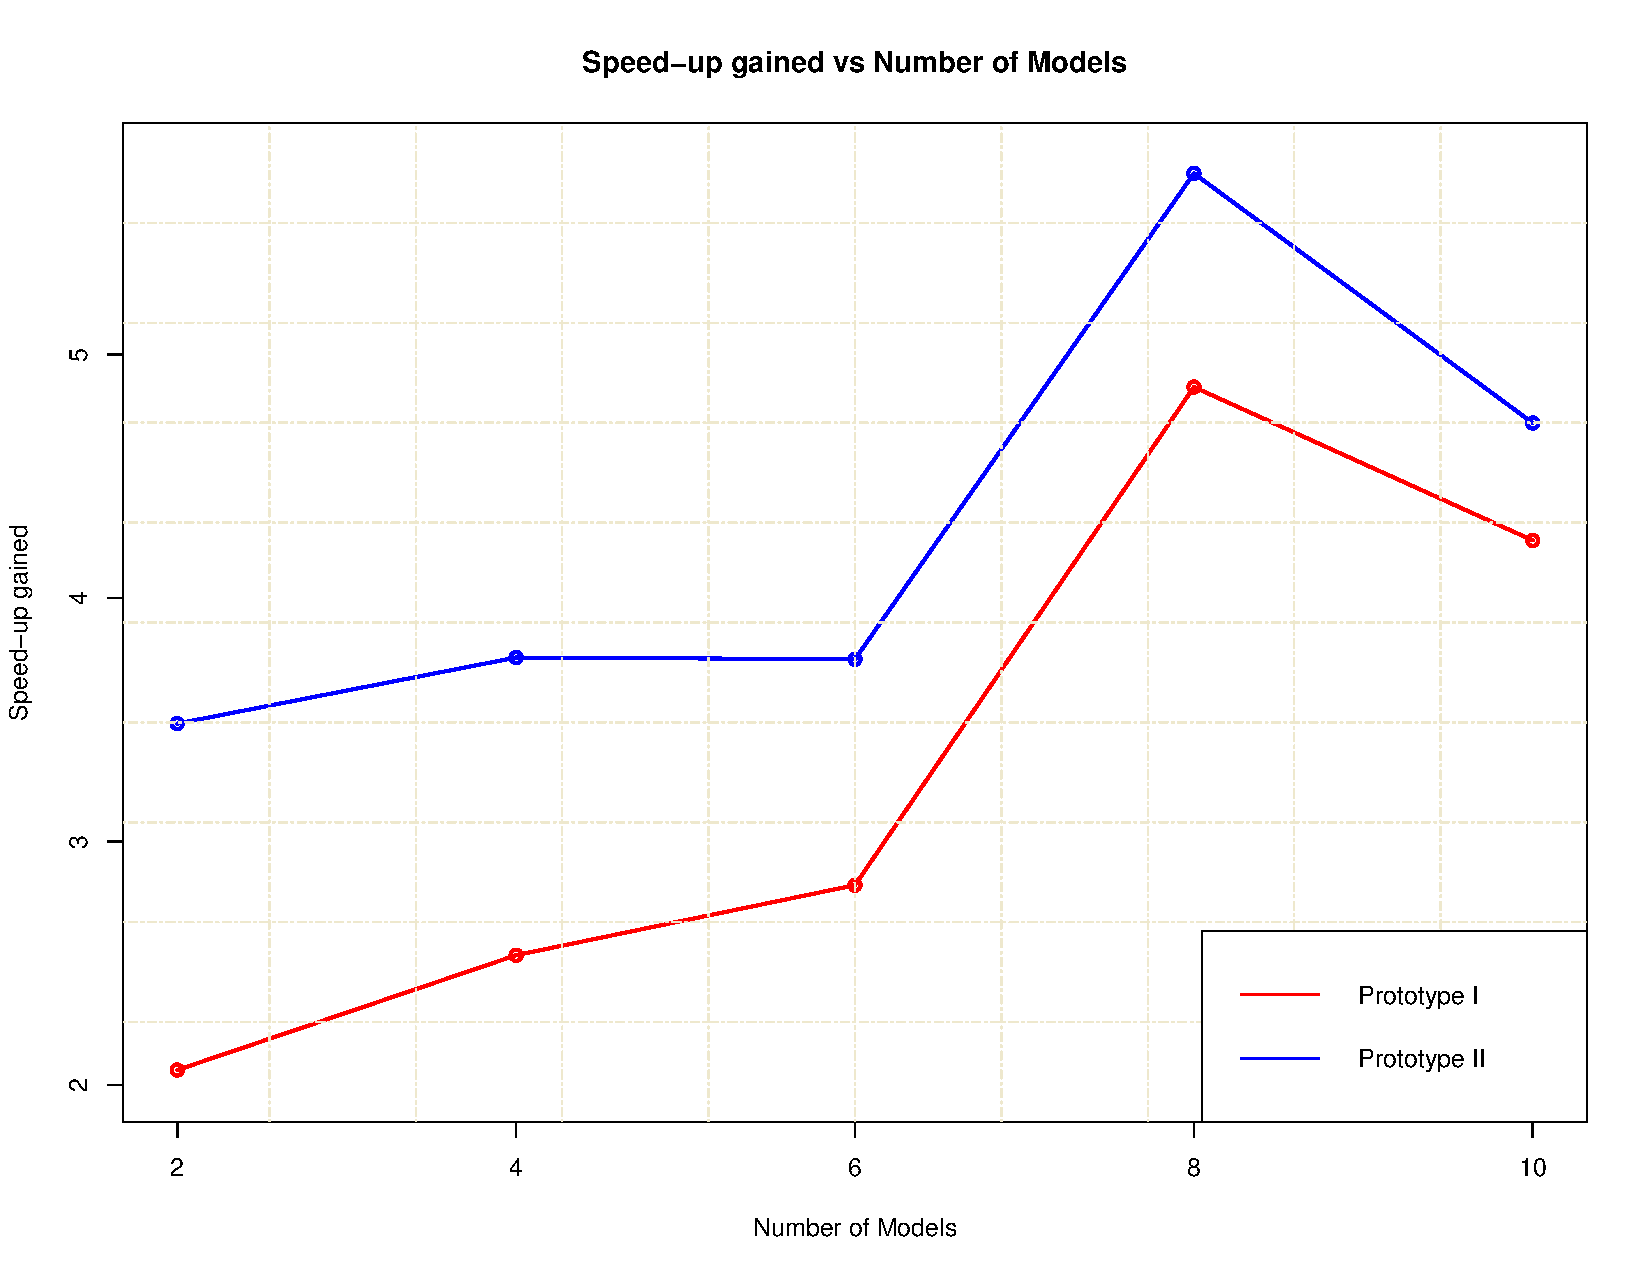
\includegraphics[width=0.9\textwidth]{SUPIPIIvsNumModGrid.pdf}
		\caption{Prototype I \& II Performance}
		\label{Fig:SUPIPIIvsNumModGrid}
\end{figure}
\end{frame}

\subsection{Prototype I vs Prototype II}
\begin{frame}
\begin{table}[]
\centering
\scalebox{0.8}{\begin{tabular}{c p{8cm} p{1cm}}
 Model
 & Test Data \\ 
\cmidrule(r){1-1}\cmidrule(lr){2-2}\cmidrule(l){3-3}
\raisebox{-\totalheight}{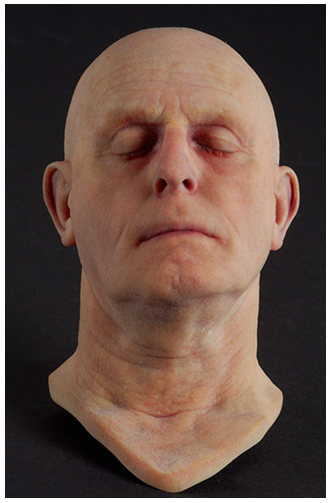
\includegraphics[width=0.2\textwidth]{Head.PNG}}
      & 
\begin{itemize}[topsep=0pt]
\item Head Model Size= 8cm
\item Resolution= \begin{math}300 \times 150 \times 470\end{math}
\item Number of Head Models= 10
\end{itemize}
\end{tabular}}
\end{table}

\begin{table}[]
\centering
\caption{Execution Time Comparison}
\label{table:ExecTimeII}
\scalebox{0.7}{\begin{tabular}{|l|l|l|l|}
\hline
\multicolumn{1}{|c|}{\textbf{\begin{tabular}[c]{@{}c@{}}Cluster\\ Size\end{tabular}}} & \multicolumn{1}{c|}{\textbf{\begin{tabular}[c]{@{}c@{}}Total Execution Time\\ (in Secs)\\  Prototype I\end{tabular}}} & \multicolumn{1}{c|}{\textbf{\begin{tabular}[c]{@{}c@{}}Total Execution Time\\ (in Secs) \\ Prototype II\end{tabular}}} & \multicolumn{1}{c|}{\textbf{\begin{tabular}[c]{@{}c@{}}Total Execution Time\\ (in Secs)\\ Native Cuttlefish\end{tabular}}} \\ \hline
3                                                                                     & 1130.51                                                                                                               & 1014.98                                                                                                               & 4790.19                                                                                                                    \\ \hline
4                                                                                     & 917.45                                                                                                                & 702.24                                                                                                                & 4790.19                                                                                                                    \\ \hline
5                                                                                     & 675.97                                                                                                                & 488.21                                                                                                                & 4790.19                                                                                                                    \\ \hline
6                                                                                     & 555.87                                                                                                                & 416.29                                                                                                                & 4790.19                                                                                                                    \\ \hline
\end{tabular}}
\end{table}
\end{frame}

\begin{frame}
\begin{figure}[!ht]
		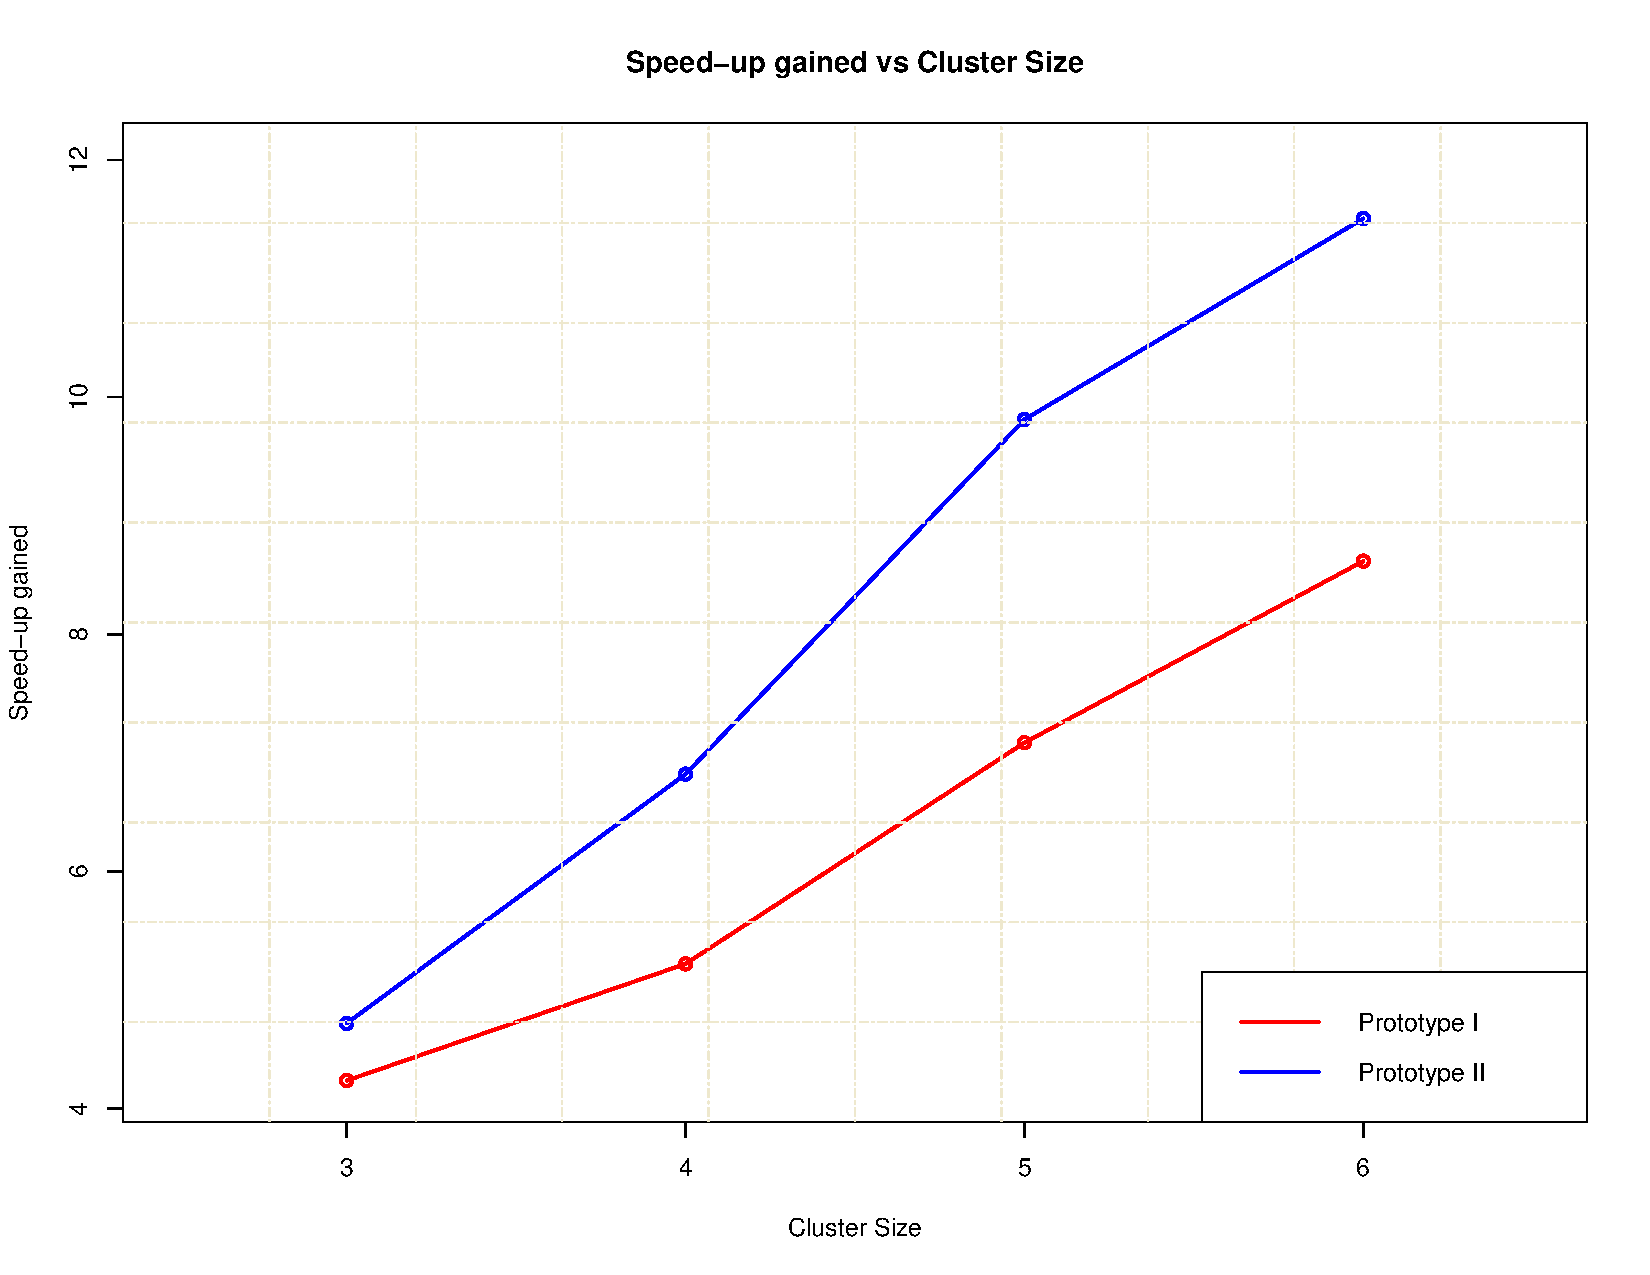
\includegraphics[width=0.9\textwidth]{SUPIPIIvsCSGrid.pdf}
		\label{Fig:SUPIPIIvsCSGrid}
\end{figure}
\end{frame}

\section*{Conclusion}
\begin{frame}
  \frametitle<presentation>{Conclusion}
	\begin{itemize}
	\item \textbf{Super-linear speed-up} can be achieved by Distributed Cuttlefish
	\begin{itemize}
	\item Cache efficiency
	\item Parallel computation
	\item Low overhead of distributed computing specific tasks 
	\end{itemize}
	\item Prototype II has a better performance than Prototype I 
	\begin{itemize}
	\item Costly serialization \& deserialization through disk I/O 
	\item Redundant input parsing
	\end{itemize}
\end{itemize} 
\end{frame}


\section*{Future Work}
\begin{frame}
  \frametitle<presentation>{Future Work}
	\begin{itemize}
	\item Use \textbf{data-driven approach} and \textbf{user-defined constraints} to form distribution function
	\item Replacing cluster computing with cloud computing
	\end{itemize} 
\end{frame}
\appendix
\section*{Appendix} 

\begin{frame}{Slave Reporter Component}
	\begin{figure}
		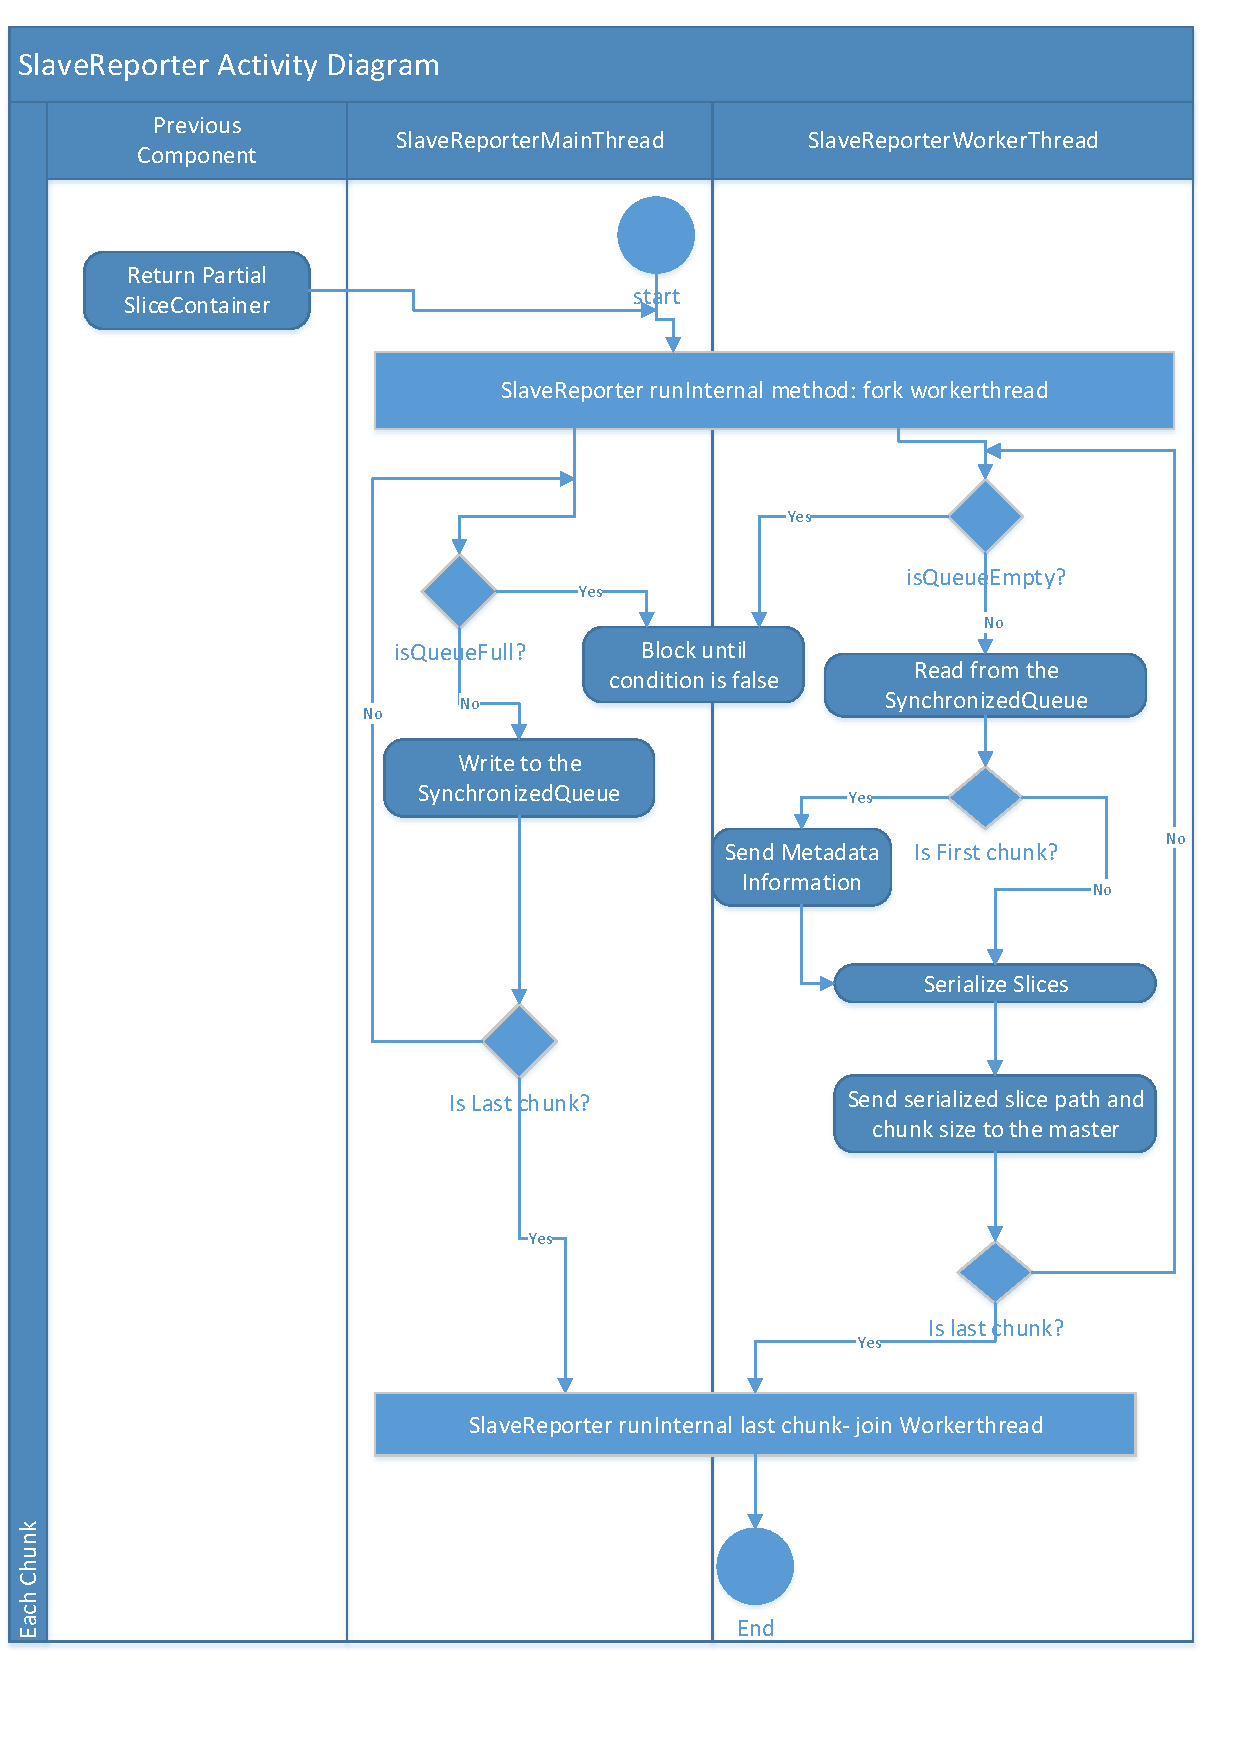
\includegraphics[width=0.50\textwidth]{SlaveReporter.pdf}
		\caption{Slave Reporter Component}
		\label{Fig:SlaveReporter}
	\end{figure}	
\end{frame}

\begin{frame}{Master Merger Component}
	\begin{figure}
		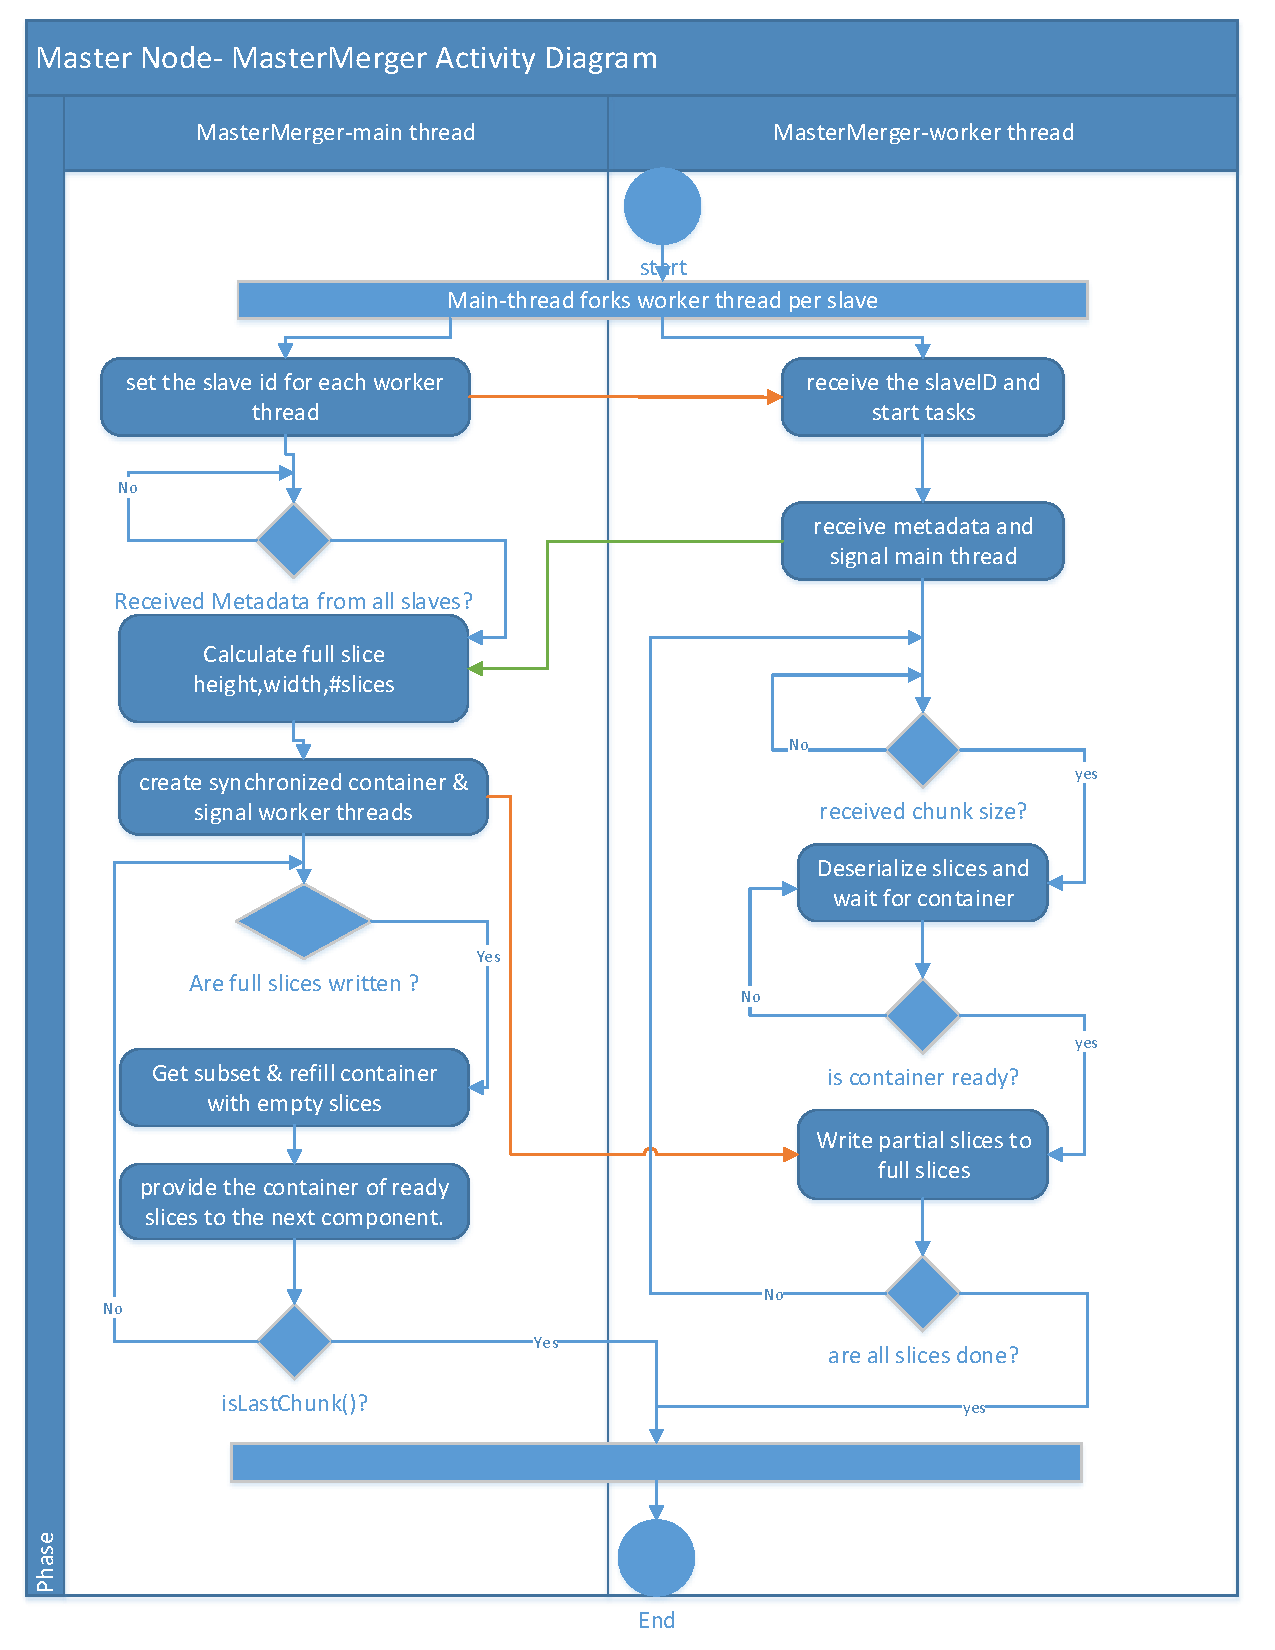
\includegraphics[width=0.55\textwidth]{MasterMerger.pdf}
		\caption{Master Merger Component}
		\label{Fig:MasterMerger}
	\end{figure}	
\end{frame}

\subsection{Profiling Prototype I}
\begin{frame}
\begin{figure}[!ht]
		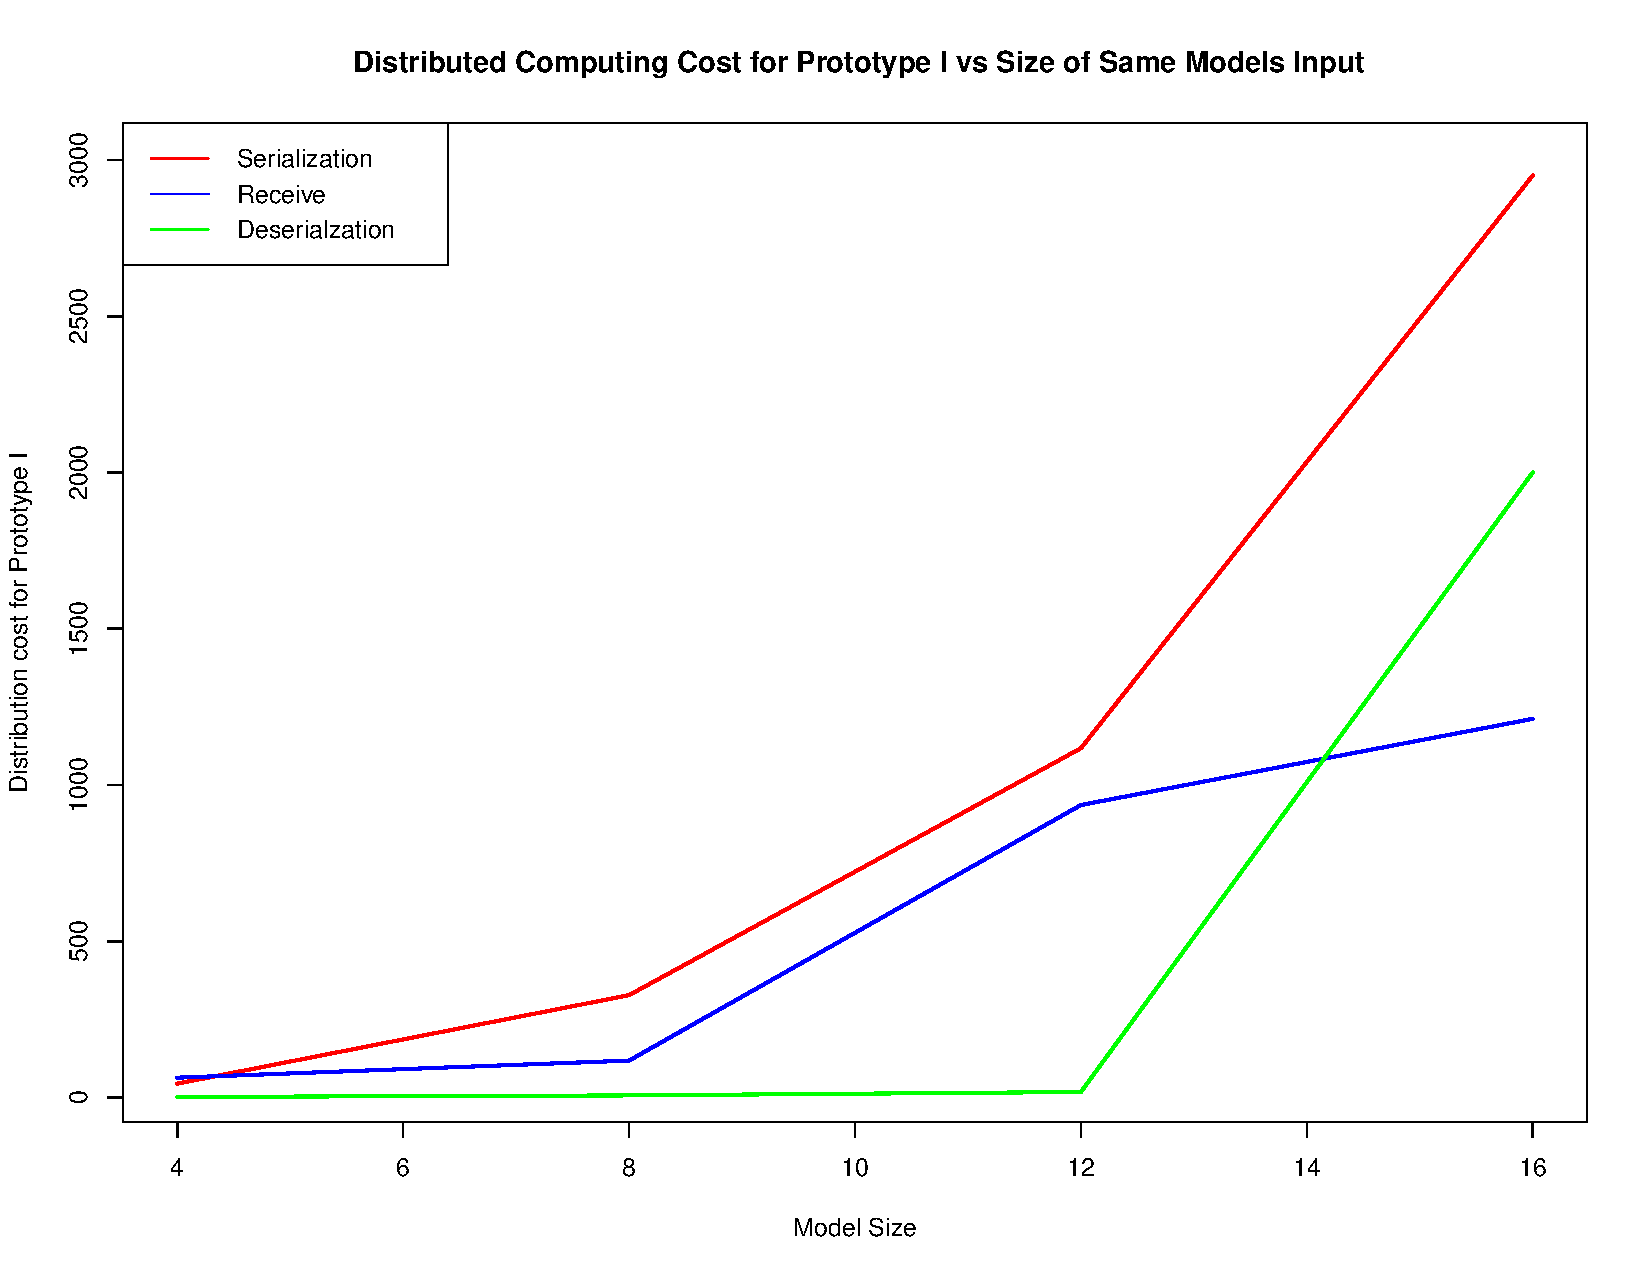
\includegraphics[width=0.9\textwidth]{DCPIvsCS.pdf}
		\caption{Profiling Prototype I}
		\label{Fig:DCPIvsCS}
\end{figure}
\end{frame}

\subsection{Profiling Prototype II}
\begin{frame}
\begin{figure}[!ht]
		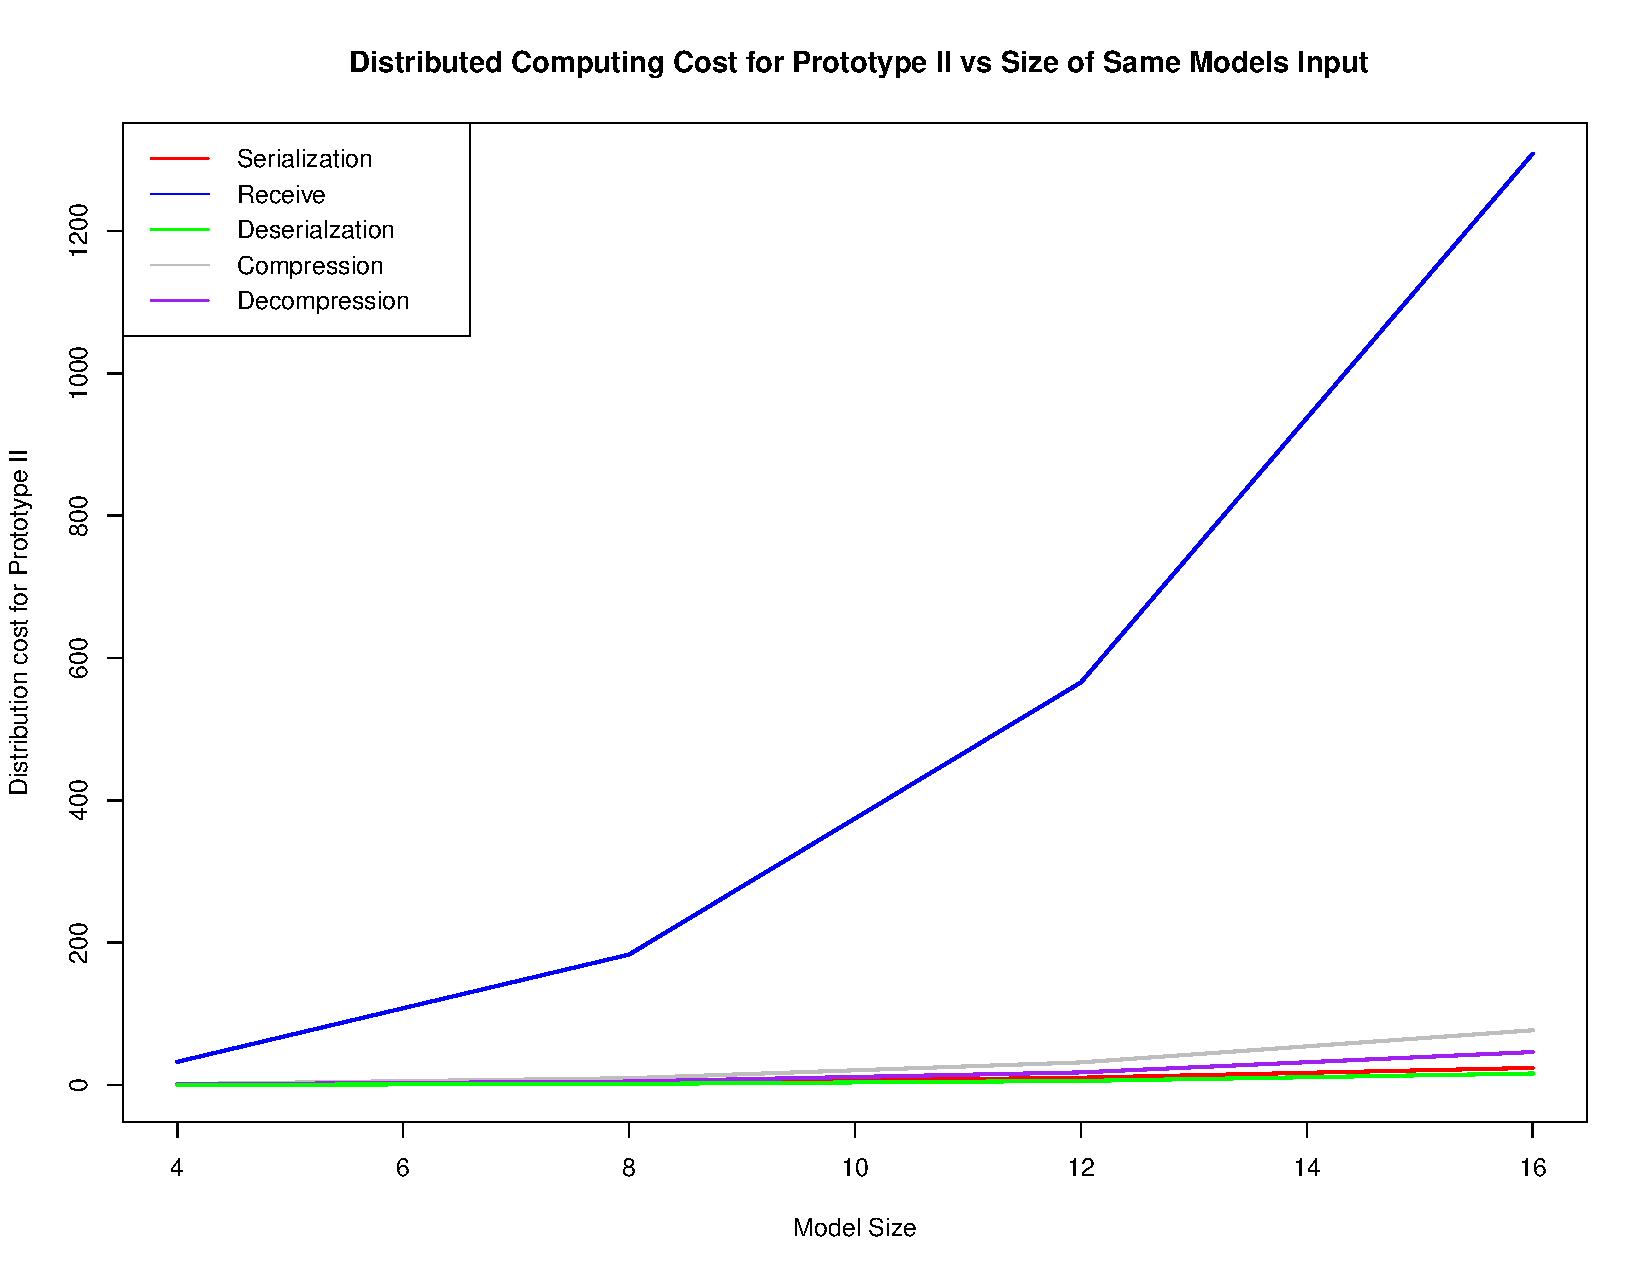
\includegraphics[width=0.9\textwidth]{DCPIIvsSize.pdf}
		\caption{Profiling Prototype II}
		\label{Fig:DCPIIvsSize}
\end{figure}
\end{frame}

\subsection{Prototype II: Design I vs Design II}
\begin{frame}
\begin{figure}[!ht]
		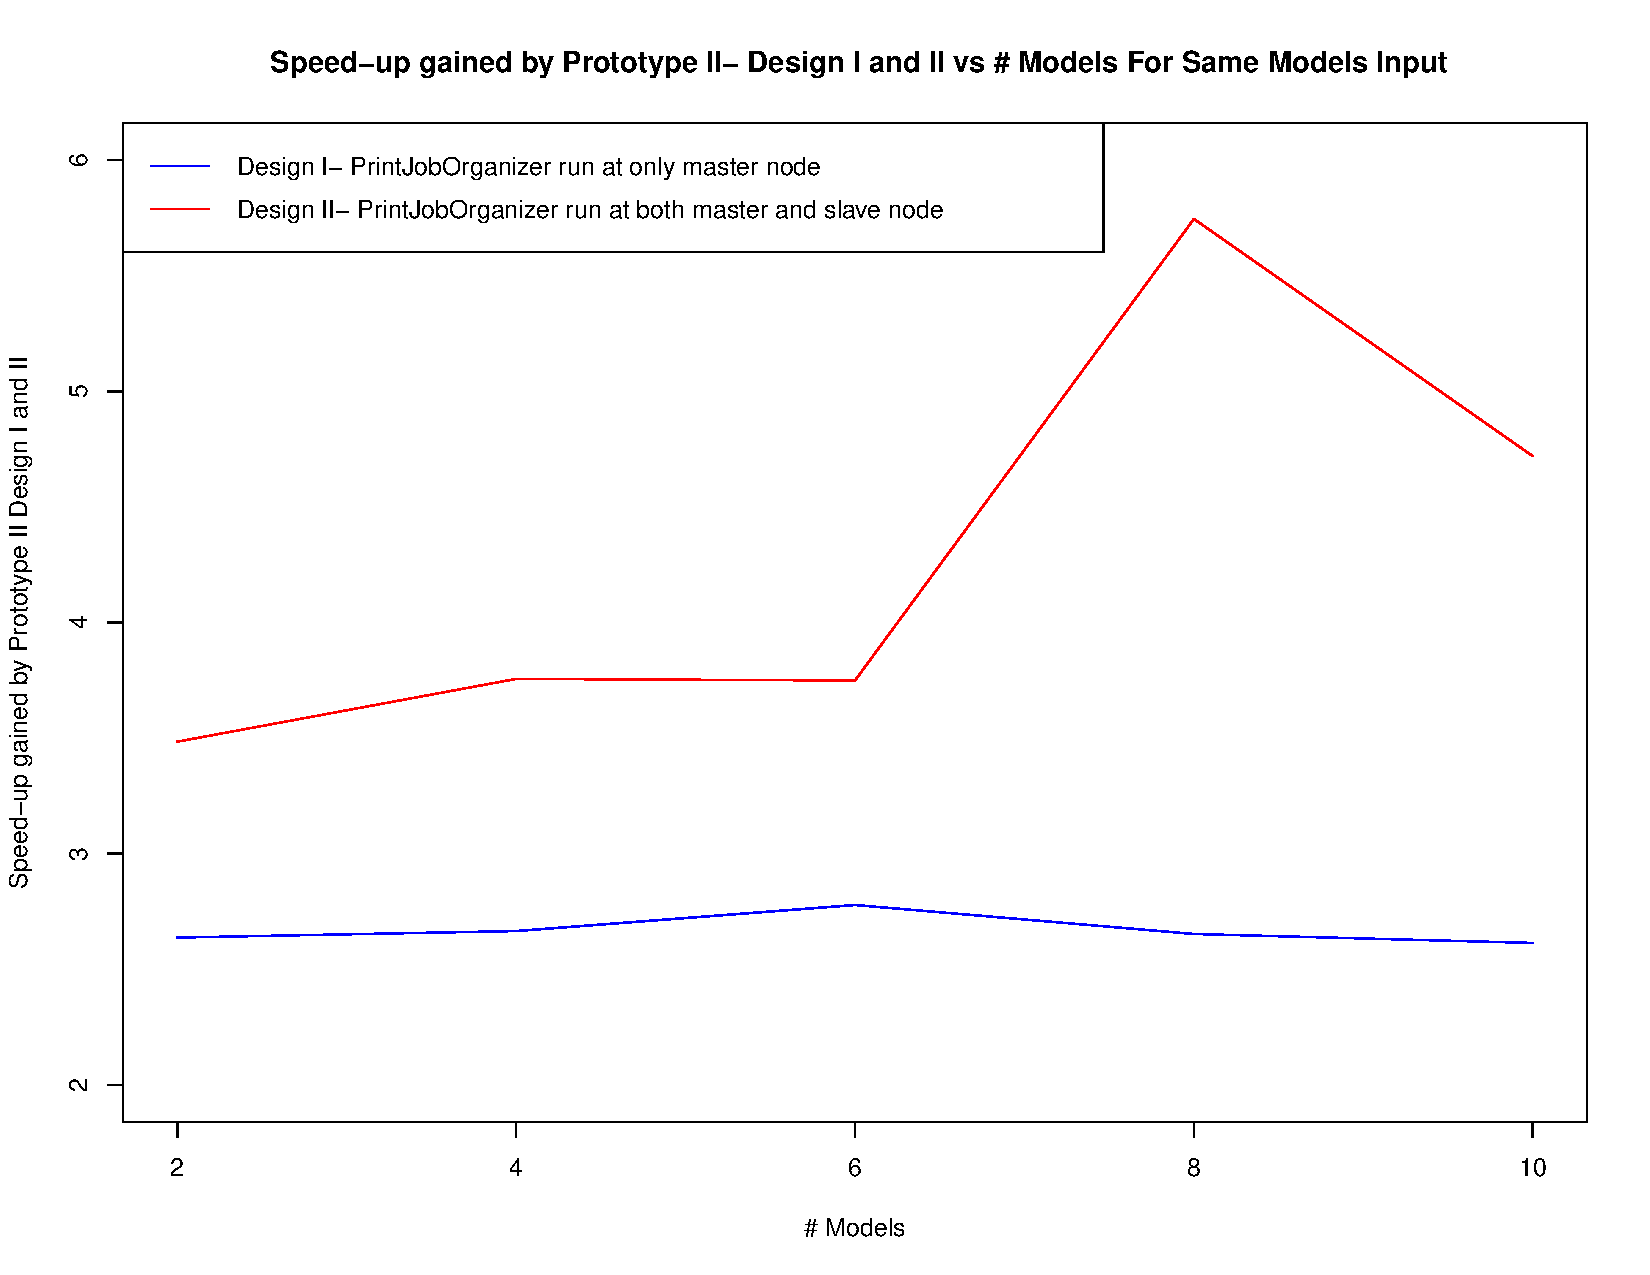
\includegraphics[width=0.9\textwidth]{SUDIDIIvsNumMod.pdf}
		\caption{Prototype II: Design I vs Design II}
		\label{Fig:SUDIDIIvsNumMod}
\end{figure}
\end{frame}

\end{document}


